\documentclass[
	12pt, 
	a4paper, 
	oneside,
	parskip=half*, % Line spacing for paragraphs
	openany,  % openany -> on which page should new chapters start
	listof=totoc, % Include listings in the table of contents
	bibliography=totoc, % adding a bibliography to the table of contents
	index=totoc, % add index directory to the table of contents
  toc=chapterentrywithdots, % Set dots in the table of contents also for chapters
  numbers=noenddot, % removes the last dot after X.X.X.
  %chapterprefix=true % changes the display of the chapter, adds "Chapter" to the chapter number
]{scrbook}


\usepackage[utf8]{inputenc}
\usepackage[english]{babel}
\usepackage{url}
\usepackage[autostyle=true,german=quotes]{csquotes}
\usepackage[T1]{fontenc}
\usepackage{pdfpages}
\usepackage{textcomp}
\usepackage{amsmath} % math environment
\usepackage{scrhack}
\usepackage{multirow}
\usepackage{diagbox}
\usepackage{makecell}
\usepackage{rotating}
\usepackage{tikz}
\usepackage{array}
\usepackage{float}
\usepackage{tabularx}
\usepackage{newtxtext}
\usepackage{booktabs}
\usepackage{longtable}
\usepackage{enumitem}
\usepackage[titles]{tocloft}
\usepackage[a4paper, margin=2.5cm]{geometry}
\usepackage{titletoc}


% ---------------------------
% |    Meta-Data for PDF    |
% ---------------------------
\usepackage[
  pdftex,
  pdfauthor={Hauke Schwarz},
  pdftitle={Thesis},
  pdfsubject={Master Thesis},
  pdfkeywords={Thesis;Template;LaTeX},
  pdfproducer={LaTeX},
  pdfcreator={pdfLaTeX},
  pdfduplex={DuplexFlipLongEdge}, %Alt.: Simplex or DuplexFlipShortEdge 
  pdflang={en},
  bookmarksopen,
  bookmarksnumbered
]{hyperref}


% ------------------
% |    Settings    |
% ------------------
\usepackage[
    backend=biber, 
    style=authoryear-icomp, % alphabetic
    citestyle=authoryear-icomp, % alphabetic, authortitle
    date=short,
    % backref=true, % Display pages on which the reference is used
    maxnames=2, % affects the cites
    maxbibnames=3, % affects the bibliography
    pagetracker=true,
    isbn=false,    
    % block=ragged, % break urls
    % firstinits=true, % shorten first names
    backrefstyle=three+ % Combine pages
]{biblatex}

% Distance between bibliographical references
\setlength{\bibitemsep}{.5em}

% Indentation after the first line
\setlength{\bibhang}{2em}

% URL in the bibliography is in angle brackets
\DeclareFieldFormat{url}{<\url{#1}>}

% break too long urls
\setcounter{biburllcpenalty}{7000}
\setcounter{biburlucpenalty}{8000}

% Source of the bibliography file
\addbibresource{literature/thesis_lib.bib}

% add comma 
\renewcommand*{\nameyeardelim}{\addcomma\space}



% graphics
\usepackage{graphicx}
\graphicspath{ {images/} }
\DeclareGraphicsExtensions{.pdf,.png,.jpg,.jpeg,.gif}

% captions
\usepackage{caption}
\usepackage{subcaption}
% Table layout
\setlength{\tabcolsep}{0.5em} % for the horizontal padding
{\renewcommand{\arraystretch}{1.2} % for the vertical padding

% Table captions
\usepackage{caption} 
\captionsetup[table]{belowskip=12pt,aboveskip=4pt}
\usepackage{diagbox}

% Rotate tables
\usepackage{rotating}
\usepackage{varwidth}

% Footnotes with tables
\usepackage{footnote}
\makesavenoteenv{figure}

% Line breaks in table cells
\newcommand{\specialcell}[2][c]{%
  \begin{tabular}[#1]{@{}c@{}}#2\end{tabular}
}

% rotate content of table cell
\def\rot{\rotatebox} % usage: \rot{angle}{content}
% You can visit this website to find more color codes for LaTeX
% http://latexcolor.com/s

\usepackage{xcolor}

% colors
\definecolor{white}{rgb}{1,1,1}
\definecolor{black}{rgb}{0,0,0}
\definecolor{middlegray}{rgb}{0.5,0.5,0.5}
\definecolor{lightgray}{rgb}{.95,.95,.95}
\definecolor{arsenic}{rgb}{0.23, 0.27, 0.29}
\definecolor{arsenicLight}{rgb}{0.20, 0.20, 0.20}
\definecolor{darkgray}{rgb}{.4,.4,.4}
\definecolor{purple}{rgb}{0.65, 0.12, 0.82}
\definecolor{orange}{rgb}{0.8,0.3,0.3}
\definecolor{yac}{rgb}{0.6,0.6,0.1}
\definecolor{green}{rgb}{.2,0.6,0.3}
\definecolor{azure}{rgb}{0.0, 0.5, 1.0}
\definecolor{editorGray}{rgb}{0.95, 0.95, 0.95}
\definecolor{editorOcher}{rgb}{1, 0.5, 0}
\definecolor{editorGreen}{rgb}{0, 0.5, 0}
\definecolor{orange}{rgb}{1,0.45,0.13}		
\definecolor{olive}{rgb}{0.17,0.59,0.20}
\definecolor{brown}{rgb}{0.69,0.31,0.31}
\definecolor{purple}{rgb}{0.38,0.18,0.81}
\definecolor{lightblue}{rgb}{0.1,0.57,0.7}
\definecolor{lightred}{rgb}{1,0.4,0.5}

\definecolor{vscodered}{HTML}{E53935}
\definecolor{vscodelightred}{HTML}{EF5350}
\definecolor{vscodeblue}{HTML}{1565C0}
\definecolor{vscodegreen}{HTML}{66BB6A}

\definecolor{lightblack}{HTML}{212121}
\definecolor{darkraspberry}{rgb}{0.53, 0.15, 0.34}

% blue hues
\definecolor{bleudefrance}{rgb}{0.19, 0.55, 0.91}
\definecolor{brandeisblue}{rgb}{0.0, 0.44, 1.0}
\definecolor{blue(ncs)}{rgb}{0.0, 0.53, 0.74}
\definecolor{coolblack}{rgb}{0.0, 0.18, 0.39}

% red hues
\definecolor{coralred}{rgb}{1.0, 0.25, 0.25}
\definecolor{darkred}{rgb}{0.55, 0.0, 0.0}

% geometry
\usepackage{geometry}
\geometry{left=25mm, right=25mm, top=25mm, bottom=30mm}

\usepackage[automark]{scrlayer-scrpage}
\pagestyle{scrheadings}
\automark*[section]{}
\clearpairofpagestyles
\ohead{\headmark} % name of the current section
\ihead{}
\ofoot{\thepage} % page number

% Define a new page style for the first page of each chapter
\deftripstyle{chapterfirst}{}{}{}{}{}{\pagemark}
\renewcommand*{\chapterpagestyle}{chapterfirst}




% footnote gap
%\addtolength{\skip\footins}{1ex}
%\addtolength{\footnotesep}{0.5ex}

% prevent footnote page break
\interfootnotelinepenalty=10000

% line spacing
\usepackage[onehalfspacing]{setspace}

% text does not have to go to the end of a page
\raggedbottom

% space before and after chapter headings
\RedeclareSectionCommand[beforeskip=0pt,afterskip=.6cm,font=\fontsize{18}{20}\selectfont]{chapter}
%\RedeclareSectionCommand[beforeskip=10pt,afterskip=.3cm,font=\fontsize{18}{25}\selectfont]{section}
%\RedeclareSectionCommand[beforeskip=10pt,afterskip=.3cm,font=\fontsize{16}{25}\selectfont]{subsection}
%\RedeclareSectionCommand[beforeskip=0pt,afterskip=.3cm,font=\fontsize{14}{25}\selectfont]{subsubsection}

\usepackage{mwe}

% chapter style
\renewcommand*{\chapterformat}{%
  \thechapter\enskip
  \textcolor{gray!70}{\rule[-\dp\strutbox]{1pt}{\baselineskip}}\enskip
}
\setkomafont{disposition}{\normalcolor\bfseries}

% adjust paragraphs
%\addtokomafont{paragraph}{\itshape}
%\setkomafont{subsubsection}{\large}
%\setkomafont{paragraph}{\normalsize\itshape}
\setkomafont{paragraph}{\normalsize}

% layout of the paragraphs
% paragraphs look like the subsubsections
\RedeclareSectionCommands[
    beforeskip=-3.25ex plus -1ex minus -0.2ex,
    afterskip=1sp, % smallest possible positive value
]{paragraph,subparagraph}

% Bold caption labels
\setkomafont{captionlabel}{\normalsize\bfseries} 
% \usepackage[font=sf]{caption} % Captions without serifs
\usepackage{listings}
\usepackage[many]{tcolorbox}

% name of listings in the toc
\renewcommand\lstlistlistingname{Listingverzeichnis}

% general settings for listing
\lstset{
    xleftmargin=1.1cm,
    belowskip=2em,
    basicstyle=\fontsize{10}{15}\ttfamily,
    basewidth  = {.5em,0.4em},
    captionpos=t,
    lineskip={2pt},
    backgroundcolor=\color{white},
    framextopmargin=6pt,
    framexrightmargin=0pt,
    framexleftmargin=0.9em,    
    framexbottommargin=6pt, 
    frame=l,
%    frame=single,        
%    frame=tb, framerule=0pt,    
    framesep=6.5mm,
    fillcolor=\color{white},
    rulecolor=\color{middlegray},
    numbers=left,
    numberstyle=\normalfont\color{middlegray},
%    numberstyle=\footnotesize,    
    numbersep=10pt,
    abovecaptionskip=10pt, %space above the caption
    belowcaptionskip=10pt, %space below the caption
    extendedchars=true,
    showstringspaces=false,
    showspaces=false,
    stepnumber=1, % the step between two line-numbers. If it is 1 each line will be numbered
    tabsize=2,
    breaklines=true,
    showtabs=false,
    upquote=true,
    % German umlauts
    literate=%
    {Ö}{{\"O}}1
    {Ä}{{\"A}}1
    {Ü}{{\"U}}1
    {ß}{{\ss}}1
    {ü}{{\"u}}1
    {ä}{{\"a}}1
    {ö}{{\"o}}1
}

% define language
\lstdefinelanguage{JavaScript}{
    keywords={typeof, new, true, false, catch, then, function, return, null, catch, switch, var, if, in, while, do, else, case, break, default},
    keywordstyle=\color{editorGreen}\bfseries,
    ndkeywords={class, export, boolean, throw, implements, import, this, const},
    ndkeywordstyle=\color{vscodeblue}\bfseries,
    identifierstyle=\color{black},
    sensitive=false,
    comment=[l]{//},
    morecomment=[s]{/*}{*/},
    commentstyle=\color{editorGreen}\ttfamily,
    stringstyle=\color{darkred}\ttfamily,
    morestring=[b]',
    morestring=[b]"
}

\lstdefinelanguage{SQL}{
    keywords={select, where, from},
    keywordstyle=\color{editorGreen}\bfseries,
    ndkeywords={},
    ndkeywordstyle=\color{vscodeblue}\bfseries,
    identifierstyle=\color{black},
    sensitive=false,
    comment=[l]{--},
    morecomment=[s]{/*}{*/},
    commentstyle=\color{editorGreen}\ttfamily,
    stringstyle=\color{darkred}\ttfamily,
    morestring=[b]',
    morestring=[b]"
}


\lstdefinelanguage{HTML5}{
  language=html,
  sensitive=true,	
  alsoletter={<>=-},	
  morecomment=[s]{<!-}{-->},
  tag=[s],
  otherkeywords={
  % General
  >,
  % Standard tags
	<!DOCTYPE,
  </html, <html, <head, <title, </title, <style, </style, <link, </head, <meta, />,
	% body
	</body, <body,
	% Divs
	</div, <div, </div>, 
	% Paragraphs
	</p, <p, </p>,
	% scripts
	</script, <script,
  % More tags...
  <canvas, /canvas>, <svg, <rect, <animateTransform, </rect>, </svg>, <video, <source, <iframe, </iframe>, </video>, <image, </image>, <header, </header, <article, </article
  },
  ndkeywords={
  % General
  =,
  % HTML attributes
  charset=, src=, id=, width=, height=, style=, type=, rel=, href=,
  % SVG attributes
  fill=, attributeName=, begin=, dur=, from=, to=, poster=, controls=, x=, y=, repeatCount=, xlink:href=,
  % properties
  margin:, padding:, background-image:, border:, top:, left:, position:, width:, height:, margin-top:, margin-bottom:, font-size:, line-height:,
	% CSS3 properties
  transform:, -moz-transform:, -webkit-transform:,
  animation:, -webkit-animation:,
  transition:,  transition-duration:, transition-property:, transition-timing-function:,
  }
}

\lstdefinestyle{html} {%
  % Code design
  keywordstyle=\color{lightblack}\bfseries,
  ndkeywordstyle=\color{lightblack}\bfseries,
  identifierstyle=\color{lightblack},
  commentstyle=\color{green}\ttfamily,
  stringstyle=\color{darkred}\ttfamily,
  % Code
  language=HTML5,
%  alsolanguage=JavaScript,
  alsodigit={.:;},	
  tabsize=2,
  showtabs=false,
  showspaces=false,
  showstringspaces=false,
  extendedchars=true,
  breaklines=true,
  % German umlauts
  literate=%
  {Ö}{{\"O}}1
  {Ä}{{\"A}}1
  {Ü}{{\"U}}1
  {ß}{{\ss}}1
  {ü}{{\"u}}1
  {ä}{{\"a}}1
  {ö}{{\"o}}1
}

\lstdefinelanguage{CSS} 
{morekeywords={color,background,margin,padding,margin,padding,font,weight,display,position,top,left,right,bottom,list,style,border,size,white,space,min,width, 	transition}, 
	sensitive=false, 
	morecomment=[l]{//}, 
	morecomment=[s]{/*}{*/}, 
	morestring=[b]", 
}

\lstdefinestyle{css} {%
  language=CSS,
  keywordstyle=\color{lightblack},
}

\lstdefinestyle{js} {
  language=JavaScript
}

\lstdefinestyle{sql} {
  language=SQL,
  keywordstyle=\color{azure}  
}

%Usage
%\begin{minipage}{\linewidth}
%\begin{lstlisting}[style=js, caption={Flux Action Creator}, label=lst:actionCreator] 
%create: function(text) {
  %AppDispatcher.dispatch({
    %type: Constants.TODO_CREATE,
    %payload: 'sample'
  %});
%},
%\end{lstlisting}
%\end{minipage}
% for the links in toc
\usepackage{hyperref}
\hypersetup{
    colorlinks,
    citecolor=black,
    filecolor=black,
    linkcolor=black,
    urlcolor=black,
    pdfstartview= % fit zoom size to the viewer
}
%\newcommand{\code}[1]{\colorbox{lightgray}{\texttt{#1}}}
%\lstinline{snippet}
%http://tex.stackexchange.com/questions/65291/code-snippet-in-text

% This "\code{my code}" can be used to highlight small code snippets in the text like names of variables or methods.
\newcommand{\code}[1]{\textcolor{black}{\texttt{#1}}}

% The "\todo{this still has to be done}" is a command that highlights todos in the text.
\newcommand{\todo}[1]{\textcolor{vscodered}{TODO: \texttt{#1}}}
% Adding package bookmark improves bookmarks handling.
% More features and faster updated bookmarks.
\usepackage{bookmark}

% \pdfbookmark[<level>]{<title>}{<dest>}

% toc is part of the bookmarks but not part the toc itself
% \pdfbookmark[section]{\contentsname}{toc}


\setlist{nosep}


\begin{document}

% Title page


% ------------------
% |    Abstract    |
% ------------------

\cleardoubleoddpage	
\pdfbookmark[section]{Abstract}{abstract} % Abstract as bookmark
\chapter*{Abstract}

\noindent
\textbf{Title:} Title 1: \\
Title 2: \\ 
\textbf{Author:} Hauke Schwarz
\vspace{1em}


Test


\vspace{3em}

\textbf{Keywords:} X, Y, Z \\
\pagenumbering{Roman}
\setcounter{page}{1}


% Abstract in Portuguese
% Acknowledgements


% ---------------------------
% |    Table of contents    |
% ---------------------------

\titlecontents{chapter}[0em] 
{\vspace{0.59em}\bfseries}  % adjust vertical space here
{\contentslabel{0em}\hspace{1em}}  % adjust label width here and add space after the label
{\hspace{0em}}  % adjust space for numberless chapters
{\titlerule*[0.8pc]{.}\contentspage}

\cleardoubleoddpage	
\pdfbookmark[section]{\contentsname}{toc} % toc is part of the bookmarks but not part the toc itself
{
  \pagestyle{empty}
  \addtocontents{toc}{\protect} 
  \tableofcontents
  \clearpage
  
}


% -----------------
% |    Indexes    |
% -----------------

\makeatletter
\renewcommand*\l@figure{\@dottedtocline{1}{0em}{2.3em}}  % For List of Figures
\renewcommand*\l@table{\@dottedtocline{1}{0em}{2.3em}}   % For List of Tables
\makeatother

\BeforeStartingTOC[lof]{\addtocontents{lof}{\protect\addvspace{3pt}}}
\BeforeStartingTOC[lot]{\addtocontents{lot}{\protect\addvspace{3pt}}}

\begingroup
\let\clearpage\relax  % Disable \clearpage
\listoffigures  % List of figures
\newpage
\listoftables  % List of tables
\endgroup

\newcommand{\listformulasname}{List of Formulas}
\newlistof{formulas}{frm}{\listformulasname}
\listofformulas

\addcontentsline{toc}{chapter}{List of Formulas}


% ------------------
% |    Acronyms   |
% ------------------

\cleardoubleoddpage	
\pdfbookmark[section]{List of Abbreviations}{loa} % List of Abbreviations as bookmark
\chapter*{List of Abbreviations}

\setlength{\LTleft}{-0.45em}  % Align the table with the left margin

\begin{longtable}{ll}
\large\textbf{Abbreviation} & \large\textbf{Definition} \\
AI & Artificial Intelligence \\
AIF360 & AI Fairness 360 \\
AUS & Automated Underwriting System \\
CA & California \\
csv & Comma-Separated Values \\
dtype & Data Type \\
EDA & Exploratory Data Analysis \\
e.g. & exempli gratia (for example) \\
ERS & Economic Research Service \\
F\&I & Fairness and Interpretations \\
FIPS & Federal Information Processing Standards \\
FPR & False Positive Rate \\
GDPR & General Data Protection Regulation \\
HMDA & Home Mortgage Disclosure Act \\
HOEPA & Home Ownership and Equity Protection Act \\
i.e. & id est (that is) \\
ibid. & ibidem (in the same place) \\
IFF & Interpretability for Fairness \\
knn & k-Nearest Neighbors \\
KPI & Key Performance Indicator \\
lei & Legal Entity Identifier \\
MAR & Missing at Random \\
Max & Maximum \\
MCAR & Missing Completely at Random \\
Min & Minimum \\
ML & Machine Learning \\
MNAR & Missing Not at Random \\
Perc. & Percentage \\
Std. & Standard Deviation \\
TPR & True Positive Rate \\
USD & United States Dollar (\$) \\
USDA & United States Department of Agriculture \\
xAI & Explainable Artificial Intelligence \\
\end{longtable}

\addcontentsline{toc}{chapter}{List of Abbreviations}


% chapters

\mainmatter
\setcounter{page}{1}
\chapter{Introduction}\label{ch:Introduction}

The Home Mortgage Disclosure Act \parencite{HMDA2022} is a dataset of publicly available U.S. mortgage data. Its nature of including demographic information including such potentially prone to discrimination like gender, race or geography of mortgage applicants alongside information on mortgage approval or disapproval have made the HMDA an often-used source for fairness research ever since its initial release.

\section{Research Objective and Significance}\label{sec:Research_Objective_and_Significance}

Fairness also is part of the scope of the \textbf{Research Question} that this thesis investigates:

\textit{“Can underlying unfairness in mortgage decision-making be detected, explained, and iteratively mitigated without sacrificing predictive performance in a subset of the 2022 HMDA dataset?”}

There already is extensive research available on the topic of fairness in algorithmic decision-making, even specifically in the field of mortgage lending.
Nevertheless, this thesis aims to make a novel contribution to this field not only by its combined analysis of Fairness and Explainability (as will be discussed in \textbf{chapter \ref{ch:Data_and_Methodology}}),
but also by the data being used: The analyses in this thesis are based on the 2022 HMDA (Home Mortgage Disclosure Act) dataset, which is a more recent data source than the academic literature analyzed relied upon.
Moreover, the dataset has been enriched with additional data sources based on geographical information, which will be discussed in \textbf{chapter \ref{subsec:Enrichment_Data}}.
This enrichment does not only serve the purpose of an improved Explainability, but also aims to tackle the issue of \textit{indirect discrimination} (i.e.\ discrimination through non-sensitive attributes like zip codes being correlated with sensitive attributes like race), 
which has been discussed in academic literature as a major issue in the field of Fairness \parencite{Mehrabi2021}.

As the Research Question states, the second important object of analysis in this thesis next to fairness will be the aspect of explainability (which will be introduced in more detail in \textbf{chapter \ref{sec:explainability}}). Only by understanding which factors drive model decisions, concrete measures to mitigate potential unfairness can be taken. Therefore, fairness and explainability are considered as two somewhat intertwined concepts in this work.

\section{Summary of the Main Findings}\label{sec:Summary_of_the_Main_Findings}

XXX Required here or doubled with abstract? XXX
\chapter{Literature Review}\label{chap:lit}

Intro here

\section{Fairness in Algorithmic Decision Making}\label{sec:fairness}

Due to the increasing use of decision-making algorithms for varying applications, the topic of \textit{Fairness} has become a heavily researched topic in the field of Machine Learning and AI.\@
While fairness concerns do not take an important role in all kinds of algorithmic decision making (some algorithms simply do not have grave enough implications to make fairness a concern, an example being buying recommendation algorithms \parencite{Marcinkevics2023}), 
they need to be focused on in applications like hiring processes or criminal justice systems, where the decisions could heavily impact individuals \parencite{Barocas2016}.
As this thesis is based on mortgage lending data and builds upon the analysis of demographic attributes like race or gender, fairness concerns are of utmost importance and will be discussed in the following sections.

\subsection{Overview of Fairness in Algorithmic Decision Making}\label{subsec:overview}

%To-Do: 
%Main issues (topical) and methods (mathematically vs. non-mathematically)
%Protected / Sensitive attributes
%Counter-Perspective (Paper Ana) - Argue that I take into consideration multiple features
%Show that my approach is novel due to new data and enrichments

\subsection{Fairness in Practice}\label{subsec:practice}

While there are a multitude of approaches to fair ML algorithms being discussed in academic literature (compare e.g.\ \cite{Mehrabi2021}), the scope of this thesis primarily includes \textit{Fairness Assessment}, i.e.\ the evaluation of the fairness of a given model, and \textit{Fair Modeling}, i.e.\ the development of fair ML algorithms.

%To-Do:
%Fair modeling (preprocessing, in-processing, postprocessing - aequitas and Choras)
%Fairness assessment (methods and metrics with formulas - aequitas, Onetto, Chouldechova, Corbett-Davies and Pessach)
%Maybe quote fair ML framework

\section{Explainability and Interpretability in Machine Learning}\label{sec:explainability}

Given the constantly increasing research into AI Interpretability and Explainability, there is surprisingly little consent on how to precisely define these concepts and how to distinguish them \parencite{Linardatos2021}. 
While both terms are used interchangeably in a multitude of publications, several studies have tried to distinguish both concepts in terms of their scope, giving rise to terms like 'xAI' (Explainable Artificial Intelligence) \parencite{Gunning2019} and occasionally also introducing related concepts like \textit{Understandability}, \textit{Comprehensibility} \parencite{Guidotti2018}, or \textit{Intelligibility} \parencite{Caruana2015}.


One of the most adapted definitions for \textit{Interpretability} has been made by Doshi-Velez and Kim, who define it as the “ability to explain or to present in understandable terms to a human” \parencite{DoshiVelez2017}. 
However, this definition does not only heavily intersect with common definitions of Explainability, it also appears to be rather general and not easily applicable in a scientific context. 
Among other unclear definitions, this has led Lipton to state that in the scientific discussion, the term Interpretability is “ill-defined”, leading to many papers in this research area only exhibiting a “quasi-scientific character” \parencite{Lipton2018}, while other authors deemed Interpretability to be a “broad, poorly defined concept” \parencite{Murdoch2019}. 
Usually, the concept of Interpretability is focused on the ability to logically comprehend the inner workings of AI algorithms, i.e.\ the user being able to predict outputs from inputs~\parencite{Kim2016}.


\textit{Explainability} or \textit{xAI} (which will be used interchangeably with the term Interpretability in this work), even though being subject to a similarly wide range of definitions, is usually defined to be more concerned with explaining the rationale behind decisions made to generate trust instead of precisely dissecting the inner workings mathematically \parencite{Gunning2019}. 
Compared to interpretable AI, which has been discussed in academic literature for a comparably longer timeframe, Explainability is a newer concept, which however seems to gather momentum in academic interest very fast, most likely due to the more and more widespread adoption of not inherently explainable Deep Learning Models \parencite{BarredoArrieta2020}.


\subsection{Inherently Interpretable Models vs. Black Box Models}\label{subsec:inherently}

Machine Learning algorithms vary in their degree of interpretability. There usually is a trade-off between their \textit{predictive accuracy} (i.e.\ how well they perform on prediction tasks) and their \textit{descriptive accuracy} (i.e.\ how well they can be understood by humans) \parencite{Murdoch2019}.
While some models, like linear regressions, are inherently interpretable, others, like Neural Networks, are considered to be 'black boxes' \parencite{Guidotti2018} or 'opaque models' \parencite{Burrell2016}, as their inner workings are not intuitively understandable for humans.
However, there is increased demand for models that have a high predictive accuracy while still being explainable due to, among others, legal requirements like the GDPR \parencite{GDPR} and ethical considerations \parencite{Guidotti2018}, leading to increased demand for explainability algorithms.

\subsection{Explainability Algorithms}\label{subsec:algorithms}

%To-Do:
%Brief methodological overview from one of the meta-studies
%Counterfactuals - see Zhou or arxiv for sources

\subsection{Application of Explainability Algorithms}\label{subsec:application}

%To-Do:
%After decision on A/B/C and model to be used: Find similar examples on similar data

\subsection{Explainability and Fairness}\label{subsec:explainability_fairness}

In order to conclude this literature review, this section will evaluate how the the concepts of Fairness and Explainability are related to each other, showing that the analysis of each adds separate value to this thesis.

Explainability and Fairness within the field of Machine Learning do not inherently share the same scope. On the one hand, as an example, Explainability is a rather objective concept, focusing on describing a model's inner workings neutrally. 
Comparing that to Fairness it becomes apparent that the latter is a more subjective concept, as it is dependent on the context and man-made definitions, which are often rooted in certain (e.g.\ political) interpretations of Fairness \parencite{Deepak2021}.
Yet, both concepts are somewhat dependent as assessing model fairness requires an understanding of the factors influencing a prediction \parencite{Zhou2022}.
Subsequently, approaches to connect both concepts have been proposed in academic literature. Two different approaches are proposed by Deepak \parencite{Deepak2021}: 
\begin{itemize}
    \item \textbf{Interpretability for Fairness (IFF)}: IFF is a framework intending to ensure that supposedly fair decisions made by AI are truly fair. The two steps in order to achieve that are \textit{clearly laying out the values supposed to adhered to} and \textit{explaining decisions made with regards to how they relate to those values}.
    \item \textbf{Fairness and Interpretations (F\&I)}: F\&I is a multi-layered approach, which, in the first step, aims to satisfy both Fairness and Interpretability requirements based on given constraints. If both criteria in combination cannot satisfyingly be met, the user needs to be informed that the model is not sufficiently interpretable, but yet adheres to at least one of the two desired properties.
\end{itemize}
However, these concepts are only stated on theoretical level without practical implications in this paper and are therefore not directly applicable for practitioners.


Following Zhou's line of reasoning \parencite{Zhou2022}, other important approaches to merge the ideas of Fairness and Explainability in academic literature include:

\textbf{Explanation as a way of guaranteeing Fairness}: ... Papers!

\textbf{Explanation as a way of shaping the perception of Fairness}: ... Papers!

\textbf{Perceived Fairness of feature properties}: ... Papers!


Another promising approach to merge the concepts of Fairness and Explainability is the identification of root-causes for a certain model behavior by identifying \textit{influential subsets} within the underlying datasets as proposed by Pradhan \parencite{Pradhan2022}\footnote{For additional information on the proposed model see https://github.com/romilapradhan/gopher}.
By combining Explainability criteria ('Why is a certain subgroup influential on the model's outcome?') with Fairness criteria ('In how far can intervention in the training data regarding these subsets improve Fairness?'), the authors manage to implement an efficient algorithm combining both concepts.

%To-Do:
%Go through sources of Zhou and list important ones
%Mention specifically newly added analysis in this thesis

\chapter{Data}\label{ch:Data}



\section{HMDA Data}\label{sec:HMDA_Data}

% Follow structure from presentation Ana: From where, why, which steps etc. - probably add in appendix the code for the enrichment?

The underlying data for this analysis was obtained \textit{\href{https://ffiec.cfpb.gov/data-browser/data/2022?category=states}{via the HMDA Data Browser}}. \@
All data used are structured, tabular data that are publicly available. Privacy concerns are not relevant, as the data is anonymized.

XXX UPDATE! XXX

The data was filtered to only include entries from California, as it is the largest state in the US and thus provides a high amount of data. 
The time frame was set to 2022, as it is the most recent year available (!!!!!!!!!!). No filter was applied to the financial institutions, as the analysis is not focused on the institutions themselves. 
The data was further filtered to only include entries for single-family homes, as these are the most common type of homes and therefore provide the most data.

The raw dataset resulting from these filters contains $XXX$ entries and $XXX$ features, with a total sum of loan applications amounting to $XXX$ USD. The column types are $XXX$ of numeric, and $XXX$ of object dtype. $XXX$ columns contain missing values. \@
Due to the size of the dataset, a step-by-step description of the analysis and all cleaning steps taken is too extensive for this thesis. Therefore, this chapter will only outline the key assumptions incorporated, decisions made, and steps taken for data analysis and cleaning. For full detail, please refer to the corresponding notebook at XXX.

After the initial EDA, the first step was to \textit{drop} all features that are not relevant for the analysis in order to reduce dimensionality and improve the model learning process. \@ 
In this initial step, the amount of features was reduced from $XXX$ to $XXX$ with the following reasoning:
\begin{itemize}
    \item \textbf{activity\_year}: Does not provide value as the year is already pre-filtered
    \item \textbf{lei}: Does not matter as all financial institutions are used
    \item \textbf{derived\_msa-md}: Does not matter as county code is the geographical variable used in the analysis
    \item \textbf{state\_code}: Does not matter as the state is already pre-filtered
    \item \textbf{census\_tract}: Not relevant for the analysis
    \item \textbf{derived\_dwelling\_category} and \textbf{construction\_method}: Do not matter as the building category is already pre-filtered
    \item All information regarding \textbf{co-applicants} were dropped as the focus is on the main applicant
    \item All available \textbf{Reasons for Denial} were dropped as the focus is only on \textit{if} the loan was approved
    \item The dataset contains geographical information based on census tracts. As, however, the analysis of geographical features will be based on county level, the \textbf{census tract} is dropped.
\end{itemize}

The dataset contains both actual information on protected attributes (e.g.\ \mbox{applicant\_ethnicity-1} to \mbox{applicant\_ethniciy-5}) and derived information that aggregate the former into one overarching category (e.g.\ \mbox{derived\_ethnicity}). 
As this analysis focuses on fairness concerns, where such protected attributes play an important role, the derived information is dropped in favor of the actual information in order to achieve a higher granularity of this important type of data.  
However, as only few applicants have made use of all the fields (for example, only 0.07\% of applicants have reported more than two ethnicities), the amount of features is reduced by only including the top two selections for each protected attribute. 
This is done in order to avoid a high amount of missing values in the dataset as well as to strike a balance between the amount of features (and therefore model performance) and the granularity of the data.

% Dropping of columns with high amount of NA including reasoning (add one or two pictures from missingno)
% Handling of other columns with a lot of NA
% Exempt: Reasoning for imputation, procedure, graphs
% Remove initial outliers to check distribution for initial imputation - comment on distributions
% Data Types: Except inferral and categorization - note: Some of the columns need further recasting (e.g. float to int / vice versa or numerical to categorical). At this stage however, the data is prepared for the next steps.


\section{Enrichment Data}\label{sec:Enrichment_Data}

% Follow structure from presentation Ana: From where, why, which steps etc. - probably add in appendix the code for the enrichment?

The enrichment data was obtained from the \textit{\href{https://www.ers.usda.gov/data-products/county-level-data-sets/}{USDA ERS page}}. All data used are structured, tabular data that are publicly available. Privacy concerns are not relevant, as the data is anonymized and aggregated. All available reports were downloaded, specifically the following datasets:

\begin{itemize}
    \item \textbf{Poverty} (2021 latest)
    \item \textbf{Population} (2022 latest)
    \item \textbf{Unemployment, and Median Household Income} (annual average 2022 unemployment and 2021 median income latest)
    \item \textbf{Education} (2017–21, 5-year average latest).
\end{itemize}

In order to clean and reshape the data in a easily analyzable format, the following steps were taken\footnote{For all detail, see the corresponding cleaning notebook at !!! XXX !!!}:
All datasets were \textit{filtered} to only contain CA county-level data, not the aggregated values for the full state of California and, in case multiple years of analysis were available, to only include the newest datapoints. 
Where there were more features available than would be useful for the analysis, the datasets were \textit{reduced} to only include the most relevant features, being:

\begin{itemize}
    \item \textbf{Poverty:} Only the percentage of the population living in poverty (PCTPOVALL\_2021) was included
    \item \textbf{Population:} Only the total population (POP\_ESTIMATE\_2022) was included
    \item \textbf{Unemployment, and Median Household Income:} The unemployment rate (Unemployment\_rate\_2022) and the median household income (Median\_Household\_Income\_2021) were included
    \item \textbf{Education:} All relative values, i.e.\ percentages of adults with their corresponding highest degrees were included.
\end{itemize}

All datasets were \textit{pivoted} in order to use the attributes as feature names and \textit{indexed} by the FIPS code and the name of the respective county. After basic \textit{checks for completeness}, the feature columns were \textit{renamed} for clarity. Finally, all datasets were \textit{merged} into a single dataframe, which was then \textit{exported} as a pickle file for further use in the analysis.

% Reasoning!

The cleaned data are \textit{complete} in a way that there are values available for all features and for all of the 58 counties. Basic summary statistics can be found in \textbf{Table \ref{tab:enrichment_summary}}. Expectedly, there is a high correlation between some of the features, see \textbf{Figure \ref{fig:CH03_Enrichment_Correlation}}.

\begin{table}[h]
    \centering
    \begin{tabularx}{\textwidth}{llllll}
    \hline
     & \textbf{Count} & \textbf{Mean} & \textbf{Std} & \textbf{Min} & \textbf{Max} \\
    \hline
    College Degree (Perc.) & 58.00 & 33.19 & 5.77 & 17.89 & 44.23 \\
    \hline
    Bachelor Degree or Higher (Perc.) & 58.00 & 28.55 & 12.27 & 11.77 & 60.15 \\
    \hline
    High School Degree (Perc.) & 58.00 & 23.77 & 5.84 & 10.17 & 38.42 \\
    \hline
    Less than High School Degree (Perc.) & 58.00 & 14.49 & 7.02 & 4.87 & 29.65 \\
    \hline
    Population (thousands) & 58.00 & 672.92 & 1,428.89 & 1.19 & 9,721.14 \\
    \hline
    Poverty Rate (Perc.) & 58.00 & 13.63 & 3.96 & 6.60 & 21.90 \\
    \hline
    Median Household Income (thousands) & 58.00 & 75.30 & 21.89 & 45.51 & 141.16 \\
    \hline
    Unemployment Rate (Perc.) & 58.00 & 4.84 & 2.07 & 2.40 & 14.70 \\
    \hline
    \end{tabularx}
    \caption{Summary Statistics of the Enrichment Data}
    \label{tab:enrichment_summary}
\end{table}

\begin{figure}[h]
    \centering
    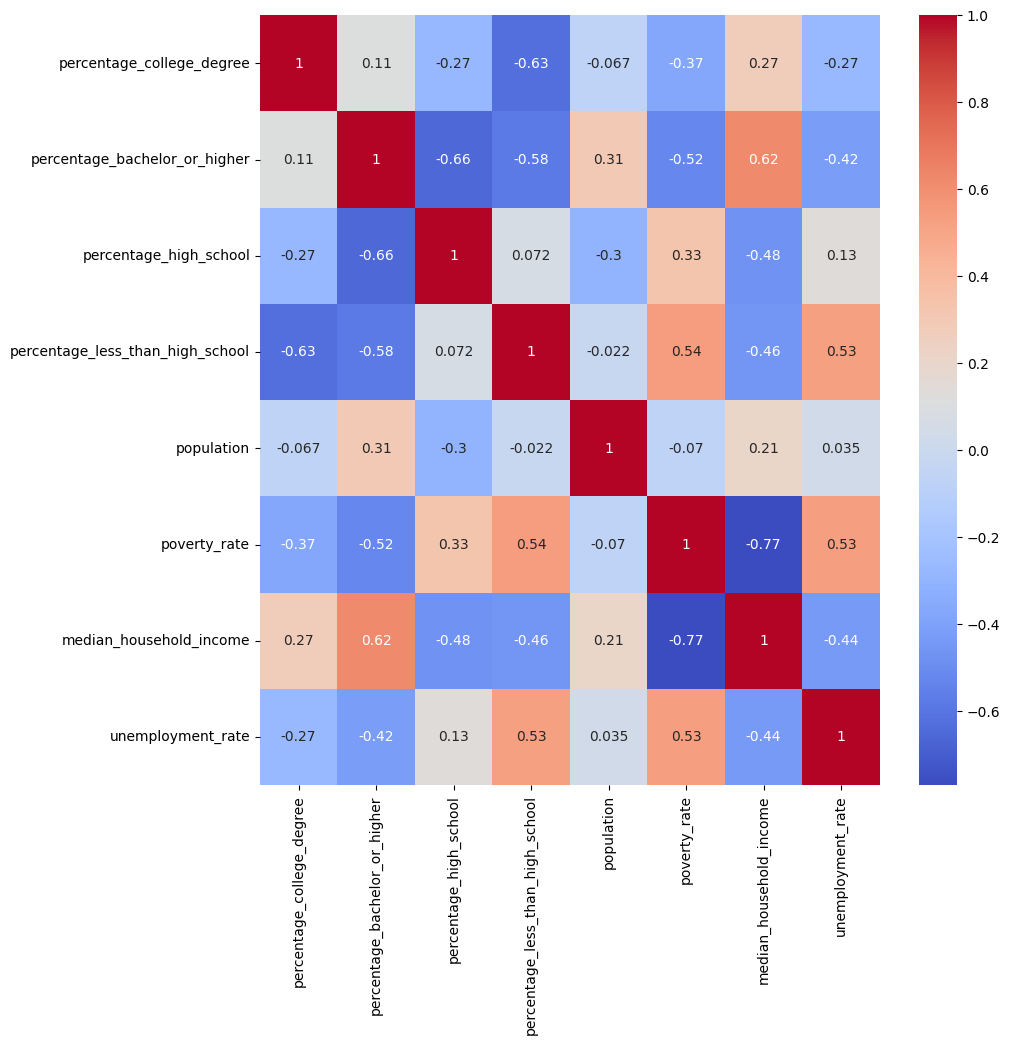
\includegraphics[width=0.7\textwidth]{images/CH03_Enrichment_Correlation.png}
    \caption{Correlation Between the Enrichment Features}
    \label{fig:CH03_Enrichment_Correlation}
\end{figure}

% appendix

\printbibliography

\end{document}